\question 下面说法正确的是( )
\par\fourch{文件系统负责文件存储空间的管理但不能实现文件名到物理地址的转换}{在多级目录结构中对文件的访问是通过路径名和用户目录名进行的}{文件可以被划分成大小相等的若干物理块且物理块大小也可以任意指定}{\textcolor{red}{逻辑记录是对文件进行存取操作的基本单位}}
\begin{solution}图4-12为文件系统模型。可将该模型分为3个层次,最底层是对象及其属性;中间层是对对象进行操纵和管理的软件集合;最高层是文件系统提供给用户的接口。其中对对象操纵和管理的软件集合这个层次,是文件管理系统的核心部分。文件系统的功能大多是在这一层实现的,其中包括对文件存储空间的管理、对文件目录的管理、用于将文件的逻辑地址转换为物理地址的机制、对文件读和写的管理,以及对文件的共享与保护等功能,所以A是错误的。在多级目录结构中,从根目录到任何数据文件,都只有一条唯一的通路。在该路径上从树的根(即主目录)开始,把全部目录文件名与数据文件名依次用``/''连接起来,即构成该数据文件的路径名。系统中的每个文件都有唯一的路径名。所以B的说法是不准确的。对文件的访问只需要通过路径名即可。对于C选项,由于物理块大小是不可以任意指定的,它必须和外存分配方式相符合,故C错误。D正确,基于文件系统的概念,可以把数据组成分为数据项、记录和文件3级。记录是一组相关数据项的集合,用于描述一个对象在某方面的属性,是文件存取的基本单位。数据项是文件可使用的最小单位。
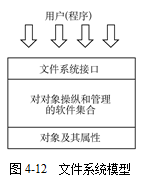
\includegraphics[width=1.48958in,height=1.89583in]{computerassets/7FB65A386B59F21177FA84BE6D2561FB.png}
\end{solution}
\question (西安电子科技大学,2006年)下列文件中属于逻辑结构的文件是
\par\twoch{连续文件}{系统文件}{散列文件}{\textcolor{red}{流式文件}}
\begin{solution}文件的逻辑结构可分为两大类,一类是有结构文件,是指由一个以上的记录构成的文件,故又把它称为记录式文件;另一类是无结构文件,是指由字符流构成的文件,故又称为流式文件。
\end{solution}
\question (武汉理工大学,2005年)对记录式文件,操作系统为用户存取文件信息的最小单位是
\par\twoch{字符}{数据项}{\textcolor{red}{记录}}{文件}
\begin{solution}记录式文件由若干个记录组成。记录是由多个字节组成的具有特定意义的信息单位,同时也是操作系统为用户存取文件信息的最小单位。记录式文件主要用于信息管理。
数据项是数据结构中讨论的最小单位,是数据记录中最基本的、不可分的有名数据单位,是具有独立含义的最小标识单位。单个数据项对用户而言是没有意义的,因此不是用户存取文件信息的单位。
\end{solution}
\question 逻辑文件的组织形式由( )决定
\par\twoch{存储介质特性}{操作系统的管理方式}{主存容量}{\textcolor{red}{用户}}
\begin{solution}文件结构包括逻辑结构和物理结构。逻辑结构是用户组织数据的结构形式,数据组织形式来自于需求,而物理结构是操作系统组织物理存储块的结构形式。因此说,逻辑文件的组织形式取决于用户,物理结构的选择取决于文件系统设计者针对硬件结构(如磁带介质很难实现链接结构和索引结构)所采取的策略(即A选项和B选项)。
\end{solution}
\question 下面对顺序文件描述不正确的选项是
\par\fourch{对记录进行批量存取是顺序文件的最佳应用场合,此时对顺序文件的存取效率是所有逻辑文件中最高的}{顺序文件的一个缺点是增加或删除一个记录都比较困难}{\textcolor{red}{查找一个记录,定长记录的顺序文件比变长记录的顺序文件开销大}}{磁带只适合存放顺序文件}
\begin{solution}选项A是顺序文件最适应的场合。
选项B说明顺序文件不易动态增长,这也是该类文件的一个弊端。解决方法是为顺序文件配置一个运行记录文件,规定每隔一定时间将运行记录文件与原来的主文件进行合并,产生一个按关键字排序的新文件。
选项C恰恰说反了,定长记录的顺序文件比变长记录的顺序文件开销小。故选择C选项。
如果对磁带进行随机访问的话,效率极低。
\end{solution}
\question (四川大学,2006年)下列关于索引表的叙述,( )是正确的
\par\fourch{索引表每个记录的索引项可以有多个}{\textcolor{red}{对索引文件存取时,必须先查找索引表}}{索引表中含有索引文件的数据及其物理地址}{建立索引表的目的之一是为减少存储空间}
\begin{solution}索引表每个记录的索引项只有一个,因此选项A错误。
对索引文件进行存取时,需要检索索引表,找到相应的表项,再利用该表项中给出的指向记录的指针值去访问所需的记录,因此B正确。
对主文件的每个记录,在索引表中都设有一个相应的表项,用于记录该记录的长度L及指向该记录的指针(指向该记录在逻辑地址空间的首址),因此C错误。
由于使用了索引表而增加了存储空间的开销,因此不会减少存储空间(此处意为存储开销),会增加存储开销。
\end{solution}
\question (南昌大学,2006年)采用直接存取法来读写磁盘上的物理记录时,效率最高的是
\par\twoch{\textcolor{red}{连续结构的文件}}{索引结构的文件}{链接结构文件}{其他结构文件}
\begin{solution}在连续文件方法下,只要知道文件在存储设备上的起始地址(首块号)和文件长度(总块数),就能很快地进行存取。适合随机存取的程度总结为:连续分配>索引分配>链接分配。
\end{solution}
\question (电子科技大学,2006年)文件的顺序存取是
\par\twoch{按终端号依次存取}{\textcolor{red}{按文件的逻辑号逐一存取}}{按物理块号依次存取}{按文件逻辑记录大小逐一存取}
\begin{solution}顺序存取文件是按其在文件中的逻辑顺序依次存取的,只能从头往下读。在4个选项中,只有逻辑号跟逻辑顺序的意思最接近,故本题选B。
\end{solution}
\question 文件系统采用两级索引分配方式,如果每个磁盘块大小为1KB,每个盘块号占4字节,则在该系统中,文件的最大长度是
\par\twoch{\textcolor{red}{64MB}}{128MB}{32MB}{以上都不对}
\begin{solution}每个磁盘块大小为1KB,每个盘块号占4字节,则一个盘块可以存放1KB/4B=256个盘块号,则二级索引文件的最大长度是256×256×1KB=64MB。
\end{solution}
\question 设某文件为索引顺序文件,由5个逻辑记录组成,每个逻辑记录的大小与磁盘块的大小相等,均为512B,并依次存放在50、121、75、80、63号磁盘块上。若要存取文件的第1569逻辑字节处的信息,则要访问(
)号磁盘块
\par\twoch{3}{75}{\textcolor{red}{80}}{63}
\begin{solution}因为1569=512×3+33。所以要访问字节的逻辑记录号为3,对应的物理磁盘块号为80。故应访问第80号磁盘。
\end{solution}
